\documentclass[a4paper, 20pt]{article}
\usepackage[english]{babel}
\usepackage{amsmath}
\usepackage{graphicx}
\usepackage{subcaption}
\usepackage{placeins}
\usepackage[T1]{fontenc}
\usepackage[utf8]{inputenc}
\usepackage{floatrow}

\author{Maarten de Jonge \\
    Inge Becht}
\date{\today}
\title{Assignment 3\\ 
Probabilistic Pose Estimation based on Topological Map}

\begin{document}
\maketitle

In this assignment it was attempted to create a topological map of 3 different
rooms using an omni camera (as was used in the previous assignment). Two
different ways of topological mapping were attempted; using wall extraction
and by using colored blobs. In the first case landmarks were determined by
finding sequences of wall parts and corridors, and in the second case the
orientation of the colored blobs were used to determine the position of the
legorobot.
These sequences, called fingerprints, could in theory be used to distinguish between
the three different rooms, as long as the fingerprints differ enough.

\section{The dataset} 
The dataset consists of multiple pictures of every room, each with a different
orientation of the robot within the room. This will create different possible
fingerprints for both the wall based topological mapping as well as the blob
based mapping. By rotating the sequences of these fingerprints it should be
clear that two fingerprints are so much alike they refer to the same room, while
reducing the noise inthe fingerprints.

\begin{figure}[!ht]
\centering
  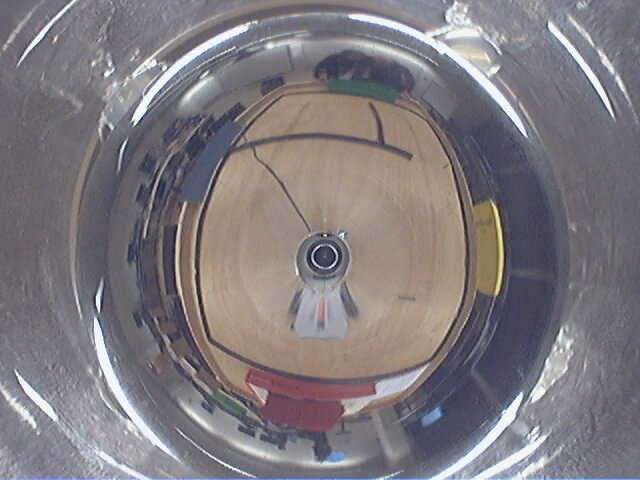
\includegraphics[width=0.5\textwidth]{data_set/2012-11-26-121531.jpg}
  \label{fig:snapshot}
  \caption{A picture from the dataset} 
\end{figure}

\section{Using wall extraction for topological mapping}
In the previous assignment we succesfully found wall points which than now are
used for finding lines.

\section{Using colored blobs for topological mapping}

\end{document}
